\clearpage
\section{Decision Rules}
\label{app:rules}

This appendix restates the decision rules of the frozen plans; nothing in it was chosen after the data were seen.

\paragraph{Primary test of order moderation (adults).} For each representation $r$, item set (8 within-domain items or all 24), and experiment $x = 1, \dots, 12$, stage~1 fits the binomial mixed model
\[
\operatorname{logit} P(y = 1) = \beta_{0x} + \beta_x\, z_d + \textstyle\sum_c \gamma_{cx}\, C_c + \sum_c \eta_{cx}\, z_d C_c + \lambda_{x,\text{level}} + u_{\text{person}},
\]
where $z_d$ is the distance standardized within representation and item set over all experiments, $C_c$ are sum-to-zero contrasts for the four teaching conditions (so $\beta_x$ is the slope averaged over conditions), and the random-effects structure is the richest rung of a fixed ladder, from (1 + $z_d$~$\mid$~person) + (1~$\mid$~image) down to (1~$\mid$~person), that converged without singularity in all 12 experiments for all 10 representations. That rung was (1~$\mid$~person) for both item sets. Stage~2 computes
\[
\hat\Delta_r = \frac{1}{6}\sum_{x \in \mathcal{E}_{31}} \hat\beta_x - \frac{1}{6}\sum_{x \in \mathcal{E}_{13}} \hat\beta_x ,
\]
the mean slope in the six experiments with the one-example trial last minus the mean in the six with it first. The two-sided $p$ value is the share of the $\binom{12}{6} = 924$ assignments of the order labels for which $|\hat\Delta^{*}| \geq |\hat\Delta_r|$ (smallest attainable value $2/924 \approx .0022$). The 95\% and 90\% intervals collect the shifts $\delta_0$ (grid step .001) for which the test applied to $\hat\Delta_r - \delta_0$ (subtracting $\delta_0$ from the slopes of the one-example-last experiments) does not reject at $\alpha = .05$ and .10, respectively. Because order is confounded with blocking, a rejection would not identify order as the cause.

\paragraph{Regions for the primary test.} With 8 items and for each margin $\delta \in \{.05, .10, .20\}$ (log odds per standard deviation), the first region that applies is: (1) opposite sign, if the 95\% upper limit is below 0; (2) smaller than $\delta$, if the 90\% interval lies inside $(-\delta, \delta)$ (two one-sided permutation tests at $\pm\delta$); (3) holds, if the 95\% lower limit is above 0 and $\hat\Delta \geq \delta$; (4) attenuated, if the 95\% lower limit is above 0 and $\hat\Delta < \delta$; (5) inconclusive otherwise. A trained representation whose positive control failed was not interpretable. With 24 items there is no margin: opposite sign (upper limit $< 0$), positive (lower limit $> 0$), or inconclusive. The positive control required a negative Wald 95\% interval for the distance slope in the 8-item model of Section~\ref{sec:adults}. Claims that hold for all representations are intersection--union tests at each representation's own 95\% level; claims that the result depends on the representation are Holm-adjusted within two families per margin (trained representations other than DINOv2-small, two tests each; the two controls, two tests each). These $p$ values were never used to choose models.

\paragraph{Geometry calibration.} For each pair of representations, Pearson's $r$ was computed between their standardized distances over the 57{,}600 rows of the 8-item data, after residualizing both on level. Representations were clustered by average linkage (UPGMA) on $1 - r$ and the tree was cut at heights .3, .5, and .7. At a given cut the grouping \emph{discriminates} only if DINOv2-base falls in the group of DINOv2-small and neither control (random ResNet-50, pixels) shares a group with a trained encoder; otherwise that cut has ``no groups'' and no claim based on groups is made. DINOv2-base grouped with DINOv2-small at all three cuts, but a control shared a group with a trained encoder at every cut (MAE with pixels at .3; both controls with CVCL and MAE at .5 and .7), so calibration failed at every cut.

\paragraph{Regions for the CIFAR analyses (H1, H2, D).} With SESOI $\in \{.10, .20, .30\}$ on $|\rho|$ or the partial $|r|$, and without multiplicity adjustment, the first region that applies is: support, if $\rho > 0$ with Mantel $p < .05$ (H1), or the distance coefficient is negative with $p < .05$ (HC3 standard errors) and the semantic-distance coefficient has $p \geq .10$ or a partial $R^2$ below one third of the distance's (H2 and D); no support, if the 95\% interval lies entirely below the SESOI (H1), or excludes every value $\leq -\mathrm{SESOI}$ or shows an opposite effect with $p < .05$ (H2 and D); inconclusive otherwise. Support therefore does not depend on the SESOI, which affects only the boundary between no support and inconclusive. The plan anticipated that, with the half-width of the H2 interval near .35 on ImageNet-HSJ, no support would be nearly unattainable. Intervals for $r$ use the Fisher $z$ transformation with standard error $1/\sqrt{n - 4}$.

\paragraph{How $p < .05$ is used.} In the first plan, the six confirmatory tests (H1 on three datasets, H2 on two, and H4) were Holm-adjusted as one family; H5 and H6 were exploratory, with Benjamini--Hochberg correction. In the multi-encoder plans, per-representation regions use unadjusted $p < .05$ (or interval limits), and Holm adjustment applies only to the union claims described above. Observation-level likelihood-ratio tests, such as those of the trial-order models in Section~\ref{sec:adults}, are exploratory and do not enter any decision.

\clearpage
\section{Post Hoc Analyses after Review}
\label{app:posthoc}

The analyses in this appendix were specified on \VcPosthocDate, after two automated external reviews of an earlier draft and after all results were known. They are outside every frozen plan, are exploratory, and are reported as they came out. All use the frozen per-trial data and embeddings, with seed 42; a model counts as converged only under the criterion of the frozen plan (no error or convergence warning and a non-singular fit).

\paragraph{By-image random slopes.} The positive-control model of Section~\ref{sec:adults} (8 within-domain items) was refitted with a by-image random slope for distance, trying in order (1 + $z_d$~$\mid$~person) + (1 + $z_d$~$\mid$~image), the same with uncorrelated image effects, and the two corresponding structures with by-person intercepts only. The first structure converged for all ten representations (Table~\ref{tab:posthoc}). The average slope stayed negative for \VcImgTrSameSignWord{} of the eight trained encoders, but the image slopes varied widely (standard deviations from \VcImgSdMin{} to \VcImgSdMax{} log odds per standard deviation of distance) and the intervals widened accordingly: the interval excluded zero for \VcImgTrExclWord{} trained encoders and included it for \VcImgTrInclList. Under this model, the reference encoder would not have passed the positive control (\VcImgRzB{} [\VcImgRzLo,~\VcImgRzHi]). The random network kept an interval below zero, and the pixel slope turned negative with an interval that included zero. Models with an additional intercept for each image--condition cell did not converge for any representation. In the superordinate-only model of Section~\ref{sec:adults}, a by-image slope for distance removed the evidence that distance improved fit given condition ($\chi^2(1) = \VcSupImgChi$, $p = \VcSupImgP$, against \VcSupFrozenDistChi{} without it), whereas condition still improved fit given distance ($\chi^2(3) = \VcSupImgCondChi$). These results do not change the frozen analyses, but they show that the within-domain association between distance and extension is less certain at the level of images than the frozen models, which estimate a single slope for all images, suggest.

\paragraph{Exemplar distances.} For a test image $x$ and teaching images $s_1, \dots, s_k$, the nearest-exemplar distance is $\min_j d(x, s_j)$ and the mean-exemplar distance is $k^{-1}\sum_j d(x, s_j)$, where $d$ is the cosine distance between single embeddings; with one teaching image both equal the centroid distance. Each was standardized and entered in place of the centroid distance, with the random-effects structure that had converged for the centroid model, so that AIC values are comparable. Across the eight within-domain items, the mean-exemplar distance fitted better than the centroid distance for \VcDmeanBetterN{} of the ten representations and the nearest-exemplar distance for \VcDminBetterN; for DINOv2-small the differences were \VcPcDmeandAIC{} and \VcPcDmindAIC{} AIC points, with slopes of \VcPcDmeanB{} and \VcPcDminB{} (centroid: \VtPcRefB). In the superordinate-only model, teaching condition improved fit given each distance for every representation (smallest $\chi^2(3) = \VcSupCondChiMinAll$). Exemplar readouts therefore do not absorb the effect of the composition of the examples. Teaching sets differed sharply in dispersion (mean pairwise distance among the three teaching images for DINOv2-small: \VcDispSub{} after same-subtype and \VcDispSup{} after broad teaching), a property that the centroid distance and these exemplar readouts do not use; models that scale generalization by dispersion were not fitted.

\begin{table}[!htbp]
\centering
\caption{Post Hoc Adult Models (Exploratory)}
\label{tab:posthoc}
\small
\setlength{\tabcolsep}{3pt}
\noindent\adjustbox{max width=\linewidth}{%
\begin{tabular}{lcccccccc}
\toprule
 & \multicolumn{2}{c}{SD of $d$} & \multicolumn{2}{c}{Distance slope (8 items)} & & \multicolumn{2}{c}{$\Delta$AIC vs.\ centroid} & \\ \cmidrule(lr){2-3}\cmidrule(lr){4-5}\cmidrule(lr){7-8}
Representation & 8 & 24 & Frozen model (refit) & By-image slopes & SD$_{\text{image}}$ & Mean & Nearest & $\chi^2_{\text{cond}}$ \\
\midrule
DINOv2-small & .296 & .219 & \ensuremath{-}3.16 [\ensuremath{-}3.30, \ensuremath{-}3.02] & \ensuremath{-}2.79 [\ensuremath{-}5.88, 0.30] & 7.76 & \ensuremath{-}153 & +1562 & 18{,}198 \\
DINOv2-base & .331 & .230 & \ensuremath{-}2.85 [\ensuremath{-}2.98, \ensuremath{-}2.72] & \ensuremath{-}2.80 [\ensuremath{-}7.40, 1.80] & 12.88 & +78 & +1465 & 17{,}145 \\
CVCL & .117 & .159 & \ensuremath{-}0.62 [\ensuremath{-}0.71, \ensuremath{-}0.52] & \ensuremath{-}1.57 [\ensuremath{-}2.44, \ensuremath{-}0.71] & 2.14 & \ensuremath{-}581 & +180 & 18{,}862 \\
SigLIP & .094 & .105 & \ensuremath{-}3.89 [\ensuremath{-}4.06, \ensuremath{-}3.71] & \ensuremath{-}5.73 [\ensuremath{-}8.02, \ensuremath{-}3.44] & 5.77 & \ensuremath{-}32 & +1672 & 14{,}072 \\
OpenCLIP & .169 & .183 & \ensuremath{-}3.99 [\ensuremath{-}4.16, \ensuremath{-}3.83] & \ensuremath{-}3.48 [\ensuremath{-}5.64, \ensuremath{-}1.31] & 5.59 & \ensuremath{-}351 & +2226 & 11{,}645 \\
ViT (supervised) & .285 & .238 & \ensuremath{-}4.30 [\ensuremath{-}4.46, \ensuremath{-}4.13] & \ensuremath{-}4.87 [\ensuremath{-}6.44, \ensuremath{-}3.30] & 3.89 & +123 & +1333 & 7{,}019 \\
ResNet-50 (supervised) & .206 & .178 & \ensuremath{-}2.65 [\ensuremath{-}2.78, \ensuremath{-}2.52] & \ensuremath{-}3.71 [\ensuremath{-}4.37, \ensuremath{-}3.05] & 1.57 & +347 & +1808 & 5{,}042 \\
MAE & .011 & .012 & \ensuremath{-}0.20 [\ensuremath{-}0.31, \ensuremath{-}0.09]$^{a}$ & 0.15 [\ensuremath{-}3.61, 3.92] & 10.10 & +15 & \ensuremath{-}380 & 18{,}628 \\
Random ResNet-50 & .00028 & .00026 & \ensuremath{-}1.10 [\ensuremath{-}1.22, \ensuremath{-}0.98] & \ensuremath{-}1.85 [\ensuremath{-}3.29, \ensuremath{-}0.40] & 3.62 & \ensuremath{-}386 & +228 & 16{,}754 \\
Pixels & .120 & .115 & 0.12 [0.04, 0.20] & \ensuremath{-}0.13 [\ensuremath{-}1.24, 0.98] & 2.73 & \ensuremath{-}112 & \ensuremath{-}60 & 18{,}837 \\
\bottomrule
\end{tabular}
}
\par\smallskip{\raggedright\footnotesize\textit{Note.} SD of $d$: raw standard deviation of the cosine distance over the trial rows of the 8-item and 24-item data, the unit of each slope. Slopes: log odds per standard deviation of distance, with Wald 95\% CIs, in the 8-item positive-control model with (1 + $z_d$~$\mid$~person) + (1~$\mid$~image) (frozen) or (1 + $z_d$~$\mid$~person) + (1 + $z_d$~$\mid$~image) (by-image slopes). Intervals are from the post hoc refit and may differ from Table~\ref{tab:v2adults} in the second decimal. SD$_{\text{image}}$: standard deviation of the by-image slopes. $\Delta$AIC: AIC with the mean- or nearest-exemplar distance minus AIC with the centroid distance (negative favors the exemplar readout). $\chi^2_{\text{cond}}$: smallest likelihood-ratio statistic for condition given distance (3 df) in the superordinate-only model across the three readouts. $^{a}$Random intercepts only, as in Figure~\ref{fig:forest}.\par}
\end{table}

\begin{figure}[!htbp]
\centering
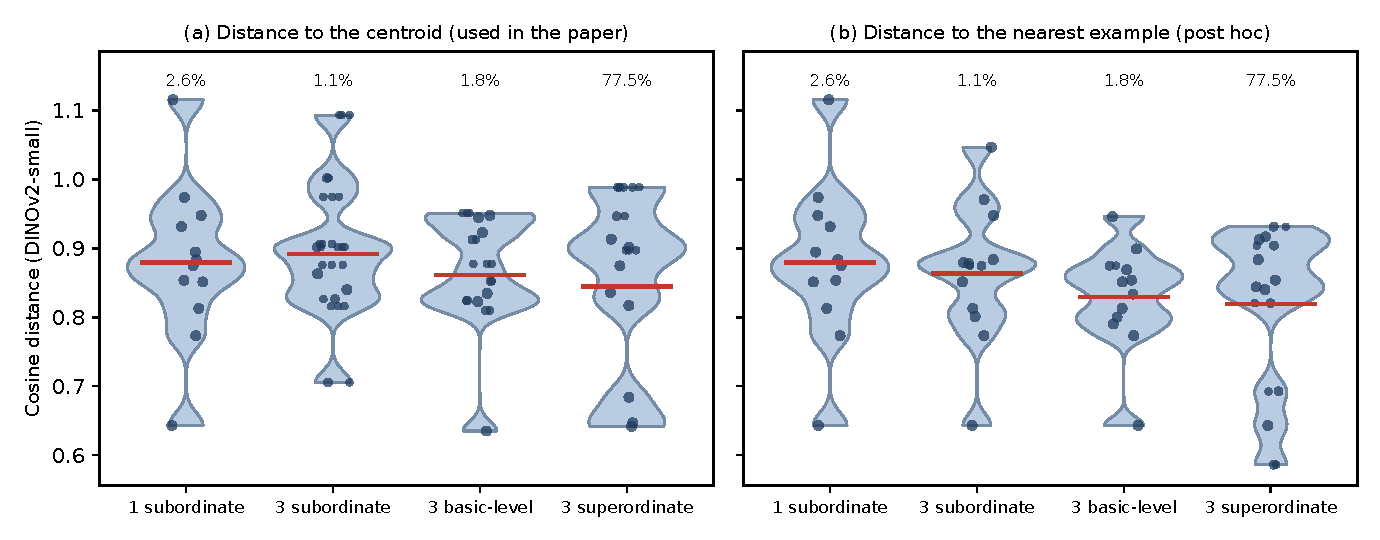
\includegraphics[width=\linewidth]{figs/fig_sup_distances.pdf}
\caption{Distances of Superordinate Test Items by Teaching Condition (DINOv2-small, Post Hoc). Distance of each superordinate test item to the centroid (left) and to the nearest teaching image (right), by teaching condition; points are the distinct image--teaching-set combinations, red lines the means, and the percentages above each violin the adults' selection rates. Mean centroid distance was \VcSupMeanSub{} (SD \VcSupSdSub) after same-subtype and \VcSupMeanSup{} (SD \VcSupSdSup) after broad teaching, while selection rose from \VcXSameSubPct\% to \VtXBroadPct\%.}
\label{fig:supdist}
\end{figure}

\paragraph{H2 estimates and detectable effects.} Table~\ref{tab:h2post} reports the H2 partial correlations for every representation with Fisher-$z$ intervals and HC3 $p$ values for the distance coefficient, the quantities behind the regions of Table~\ref{tab:v2agentsH}. With $n = 61$ and 32 pairs, the half-width of the 95\% interval at $r = 0$ is \VcMdeHalfThings{} and \VcMdeHalfHsj, and the smallest correlation detectable with 80\% power at two-sided $\alpha = .05$ is \VcMdeThings{} and \VcMdeHsj{}. The descriptive analysis on all mapped pairs (\VcHtwoAllThingsN{} for THINGS and \VcHtwoAllHsjN{} for ImageNet-HSJ) gave negative correlations for every representation, but its pairs share categories and are not independent, so it is not a test.

\begin{table}[!htbp]
\centering
\caption{Human Distance and Learner Difficulty (H2) by Representation (Post Hoc Summary)}
\label{tab:h2post}
\small
\setlength{\tabcolsep}{3pt}
\noindent\adjustbox{max width=\linewidth}{%
\begin{tabular}{lcccccc}
\toprule
 & \multicolumn{3}{c}{THINGS ($n = 61$)} & \multicolumn{3}{c}{ImageNet-HSJ ($n = 32$)} \\ \cmidrule(lr){2-4}\cmidrule(lr){5-7}
Representation & $r$ [95\% CI] & $p$ & all pairs $r$ & $r$ [95\% CI] & $p$ & all pairs $r$ \\
\midrule
DINOv2-small & \ensuremath{-}.10 [\ensuremath{-}.34, .16] & .374 & \ensuremath{-}.20 & \ensuremath{-}.41 [\ensuremath{-}.67, \ensuremath{-}.07] & .039 & \ensuremath{-}.18 \\
DINOv2-base & \ensuremath{-}.17 [\ensuremath{-}.41, .09] & .164 & \ensuremath{-}.22 & \ensuremath{-}.40 [\ensuremath{-}.66, \ensuremath{-}.05] & .052 & \ensuremath{-}.21 \\
CVCL & .08 [\ensuremath{-}.17, .33] & .561 & \ensuremath{-}.06 & \ensuremath{-}.39 [\ensuremath{-}.65, \ensuremath{-}.04] & .052 & \ensuremath{-}.05 \\
SigLIP & \ensuremath{-}.16 [\ensuremath{-}.40, .10] & .144 & \ensuremath{-}.27 & \ensuremath{-}.50 [\ensuremath{-}.73, \ensuremath{-}.18] & .011 & \ensuremath{-}.12 \\
OpenCLIP & \ensuremath{-}.20 [\ensuremath{-}.43, .06] & .088 & \ensuremath{-}.30 & \ensuremath{-}.45 [\ensuremath{-}.70, \ensuremath{-}.12] & .022 & \ensuremath{-}.13 \\
ViT (supervised) & \ensuremath{-}.08 [\ensuremath{-}.33, .17] & .476 & \ensuremath{-}.12 & \ensuremath{-}.39 [\ensuremath{-}.65, \ensuremath{-}.04] & .069 & \ensuremath{-}.24 \\
ResNet-50 (supervised) & \ensuremath{-}.04 [\ensuremath{-}.29, .22] & .749 & \ensuremath{-}.14 & \ensuremath{-}.38 [\ensuremath{-}.65, \ensuremath{-}.03] & .058 & \ensuremath{-}.10 \\
MAE & .13 [\ensuremath{-}.12, .38] & .229 & \ensuremath{-}.07 & \ensuremath{-}.27 [\ensuremath{-}.57, .10] & .131 & \ensuremath{-}.07 \\
Random ResNet-50 & \ensuremath{-}.06 [\ensuremath{-}.31, .20] & .655 & \ensuremath{-}.08 & \ensuremath{-}.35 [\ensuremath{-}.63, .00] & .032 & \ensuremath{-}.03 \\
Pixels & .08 [\ensuremath{-}.17, .33] & .487 & \ensuremath{-}.07 & \ensuremath{-}.28 [\ensuremath{-}.58, .08] & .143 & \ensuremath{-}.06 \\
\bottomrule
\end{tabular}
}
\par\smallskip{\raggedright\footnotesize\textit{Note.} $r$: partial correlation of human distance with naming accuracy, controlling semantic distance, on the covered pairs of the 100 dissociation pairs; 95\% CI from the Fisher $z$ transformation. $p$: HC3 $p$ value of the distance coefficient, used by the unadjusted regions. All pairs $r$: the same partial correlation over all mapped pairs, descriptive.\par}
\end{table}
